\section*{12 - 15. Support Vector Machines, Duality and Kernels}
\textbf{Source:} Hastie, Tibshirani, Friedman - The Elements of Statistical Learning
\subsection*{Separating Hyperplanes}
\begin{figure}[H]
    \centering
    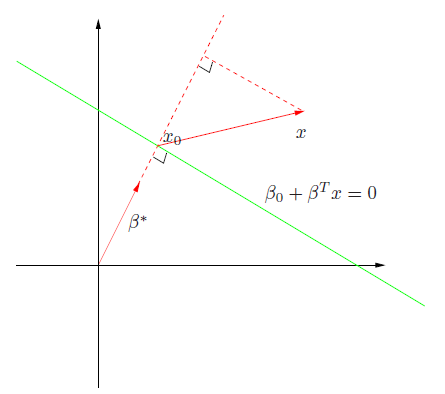
\includegraphics[scale=1]{figures/hyperplane}
\end{figure}
\begin{itemize}
    \item 
        Hyperplane $L$ is defined by $f(x) = \beta_0 + \beta^T x = 0$
    \item
        Properties:
        \begin{itemize}
            \item
                For any two points $x_1$ and $x_2$ lying in L, $\beta^T (x_1-x_2)=0$, and hence $\beta^* = \beta / \norm{\beta}$ is the vector normal to the surface of L
            \item
                For any point $x_0$ in $L$, $\beta x_0 = -\beta_0$
            \item
                The signed distance of any point $x$ in $L$ is given by
                $$\beta^{*T} (x - x_0) = \ffrac{1}{\norm{\beta}} (\beta^T x + \beta_0)$$
        \end{itemize}
        Hence $f(x)$ is proportional to the signed distance from $x$ to the hyperplane defined by $f(x) = 0$
\end{itemize}

\subsection*{Optimal Separating Hyperplanes}
\begin{itemize}
    \item
        Optimization problem:
        $$ \underset{\beta, \beta_0, \norm{\beta}}{max} M$$
        $$ \text{subject to } y_i (x_i^T)\beta + \beta_0 \geq M, i=1,\dots,N$$ 
    \item
        The set of conditions ensure that all the points are at least a signed distance $M$ from the decision boundary
    \item
        We can get rid of the $\norm{\beta} = 1$ constraint by replacing the condition with 
        $$\ffrac{1}{\norm{\beta}} y_i (x_i^T)\beta + \beta_0 \geq M$$
        or equivalently
        $$y_i (x_i^T)\beta + \beta_0 \geq M \norm{\beta}$$
    \item
        Since for any $\beta$ and $\beta_0$ satisfying these inequalities, any positively scaled multiple satisfies them too, we can arbitratily set $\norm{\beta} = 1/M$. The following then is an equivalent formulation:
        $$\underset{\beta, \beta_0}{min}\ffrac{1}{2} \norm{\beta}^2$$
        $$\text{subject to } y_i (x_i^T)\beta + \beta_0 \geq 1$$
    \item
        The constraints define a margin around the decision boundary of thickness $1/\norm{\beta}$. We choose $\beta$ and $\beta_0$ to maximize its thickness.
    \item
        The Lagrange (primal) function to be minimized w.r.t $\beta$ and $\beta_0$ is 
        $$L_P = \ffrac{1}{2} \norm{\beta}^2 - \sum_1^N \alpha_i [y_i(x_i^T \beta + \beta_0) -1]$$
    \item
        Setting the derivatives to zero, we obtain:
        $$ \beta = \sum_{i=1}^{N} \alpha_i y_i x_i$$
        $$ 0 = \sum_{i=1}^N \alpha_i y_i $$
    \item
        Substituting these into the Lagrange function, we obtain the so-called Wolfe dual:
        $$ L_D = \sum_{i=1}^{N} \alpha_i - \ffrac{1}{2} \sum_{i=1}^{N} \sum_{k=1}^{N} \alpha_i \alpha_k y_i y_k x_i^T x_k$$
        $$ \text{subject to } \alpha_i \geq 0 \text{ and } \sum_{i=1}^{N} \alpha_i y_i = 0$$
    \item
        This is a simpler convex optimization problem
    \item
        The solution must satisfy the Karush-Kuhn-Tucker conditions, including complementary slackness:
        $$\alpha_i [y_i (x_i^T \beta + \beta_0) - 1] = 0 \forall i$$
    \item
        From this we can see that:
        \begin{itemize}
            \item
                if $\alpha_i > 0$, then $y_i (x_i^T \beta + \beta_0) = 1$, or in other words, $x_i$ is on the boundary of the margin
            \item
                if $y_i(x_i^T \beta + \beta_0) > 1$, $x_i$ is not on the boundary of the margin and $\alpha_i = 0$
        \end{itemize}
    \item
        From the above equation $\beta = ...$ we see that the soultion vector $\beta$ is defined in terms of a linear combination of the support vectors $x_i$
    \item
        The decision function of the Optimal Margin Classifier is defined by $G(x) = sign(f(x))$\\

    \item
        For the soft margin case, we have the following problem
        $$\underset{\beta, \beta_0}{min}\ffrac{1}{2} \norm{\beta}^2 + \mu \sum_i \xi_i$$
        \begin{align*}
            \text{subject to } & y_i (x_i^T)\beta + \beta_0 \geq 1\\
            & -\xi_i \leq 0
        \end{align*}
        where $\xi_i$ are called slack variables
    \item
        Big cost parameter $\mu$ makes margin smaller (focuses attention more on correctly classified points near the decision boundary), while smaller values make it larger (involves data further away)
\end{itemize}

\subsection*{SVM and Kernels}
\begin{itemize}
    \item
        Support vector classifier so far is restricted to linearly seperable classes
    \item
        One way to solve this would be to use basis expansion (transform into higher dimensional space) to make the classes linearly seperable, where the downside is the increasingly high computation cost
    \item
        Observation: inside the solution of optimization problem $x_i$'s only occur as inner products
    \item
        Applying the basis function $h$ we get:
        $$ L_D = \sum_{i=1}^N \alpha_i - \ffrac{1}{2} \sum_{i=1}^N \sum_{i'=1}^N \alpha_i \alpha_{i'} y_i y_{i'} \inner{h(x_i), h(x_i')}$$
        and
        $$ f(x) = h(x)^T \beta + \beta_0 = \sum_{i=1}^{N} \alpha_i y_i \inner{h(x), h(x_i)} + \beta_0$$
    \item
        We need not speficy the transformation $h(x)$ at all, but require only knowledge of the kernel function
        $$ K(x, x') = \inner{h(x), h(x')}$$
        that computes the inner products in the transformed space. K should be a symmetric positive (semi-) definite function
    \item
        Three popular choices for $K$ in the SVM literature are:
        \begin{itemize}
            \item
                $d$-th Degree polynomial: $K(x, x') = (1 + \inner{x, x'})^D$
            \item
                Radial basis: $K(x,x') = exp(-\varphi \norm{x-x'}^2)$
            \item
                Neural network: $K(x, x') = tanh(\kappa_1 \inner{x, x'} + \kappa_2)$
        \end{itemize}
\end{itemize}

\subsection*{SVM for Regression}
\begin{itemize}
    \item
        Linear regression model $f(x) = x^T \beta + \beta_0$
    \item
        To estimate $\beta$, we consider the minimization of
        $$H(\beta, \beta_0) = \sum_{i=1}^N V(y_i - f(x_i)) + \ffrac{\lambda}{2} \norm{\beta}^2$$
        where 
        \[ V_{\epsilon}(r)=
        \begin{cases}
            0 & \text{if } \norm{r} < \epsilon\\
            |r| - \epsilon &\text{otherwise}
        \end{cases}
        \]
    \item
        $\epsilon$ is parameter of loss function, $\lambda$ is a more traditional regulariatzion parameter
    \begin{figure}[H]
        \centering
        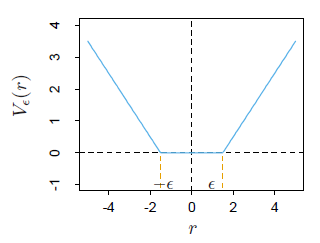
\includegraphics[scale=1]{figures/svm_regression}
    \end{figure}
\end{itemize}

\subsection*{Kernel PCA}
\begin{itemize}
    \item
        PCA:
        \begin{itemize}
            \item 
                Compute the scatter matrix (covariance matrix)
                $$\Sigma = \ffrac{1}{m} \sum_{i=1}^{m} x_i x_i^T$$
            \item
                Compute the eigenvectors and eigenvalues
                $$\Sigma e_i = \lambda_i e_i$$
        \end{itemize}
    \item
        The eigenvetors $e_i$ span the same space as the feature vectors
    \item
        Each eigenvector $e_i$ can be written as a linear combination of feature vectors
        $$e_i = \sum_{k} a_{i,k} x_k$$
    \item
        Reformulation:
        $$ \Sigma e_i = \lambda_i e_i$$
        $$ (\ffrac{1}{m} \sum_{j=1}^{m} x_j x_j^T)\cdot \sum_k a_{i,k} x_k = \lambda_i \sum_k a_{i,k}x_k$$
        $$ \sum_{j,k} a_{i,k} x_j x_j^T x_k = m \cdot \lambda_i \sum_k a_{i,k} x_k$$
    \item
        Multiply by $x_l^T$:
        $$ \sum_{j,k} a_{i,k} x_l^T x_j x_j^T x_k = m \cdot \lambda_i \sum_k a_{i,k} x_l^T x_k$$
    \item
        For any kernel $k(x,x')$, we get the key equation for Kernel PCA
        $$ \sum_{j,k} a_{i,k} k(x_l,x_j) k(x_j,x_k) = m \cdot \lambda_i \sum_k a_{i,k} k(x_l,x_k)$$
    \item
        This can be written in matrix notation using a matrix $K \in \mathbb{R}^{m\times m}$ and a vector $a_i = (a_{i,1}, a_{i,2} , \dots, a_{i,m})^T$
        $$K a_i = m \lambda_i a_i$$
    \item
        Kernel PCA (and thus classical PCA) can be computed by solving an eigenvector/-value problem for an $(m \times m)$-matrix, where $m$ is the cardinality of the training feature set
    \item
        The principal components cannot be computed easily, because only the kernel is known, but not $\phi(x)$
    \item
        However the projection $c$ of the transformed feature vector $\phi(x)$ on principal component $e_i = \sum_k a_{i,k} \phi(x_k)$ is easily computed by
        $$c = \phi(x)^T e_i = \dots = \sum_k a_i,k k(x,x_k)$$
    \item
        Transformed features have to have zero mean, which can be achieved by modifying $K$
\end{itemize}

\subsection*{Duality}
\subsubsection*{The Lagrange dual function}
\begin{itemize}
    \item
        Primal optimization problem:
        \begin{align*}
            minimize \; \; & f_0(x)\\
            subject \; to \; \; & f_i(x) \leq 0 \\ %\;\; \forall i=1, \dots, m
            & h_i(x) = 0 \\
        \end{align*}
        Optimal value: $p^*$\\
        We do not assume the problem is \textbf{convex}.
    \item
        Lagrangian:
        $$ L(x, \lambda, v) = f_0(x) + \sum_{i=1}^{m} \lambda_i f_i(x) + \sum_{i=1}^{p} v_i h_i(x)$$
        The vectors $\lambda$ and $v$ are called the dual variables.
    \item
        Lagrange dual function:
        $$ g(\lambda, v) = inf(L(x, \lambda, v)) = inf(f_0(x) + \sum_{i=1}^{m} \lambda_i f_i(x) + \sum_{i=1}^{p} v_i h_i(x))$$
        The dual function is \textbf{concave}, even when the problem isn't.
        The dual function yields lower bounds on the optimal value $p^*$ of the problem: For any $\lambda \geq 0$ and any $v$ we have $g(\lambda, v) \leq p^*$.
\end{itemize}
\subsubsection*{The Lagrange dual problem}
\begin{itemize}
    \item
        Lagrange dual problem:
        \begin{align*}
            maximize \;\; & g(\lambda, v)\\
            subject \; to \; \; & \lambda \geq 0
        \end{align*}
        $(\lambda^*, v^*)$ is refered to as dual optimal.\\
        The Langrange dual problem is a convex optimization problem, since the objective to be maximized is concave and the constraint is convex. This is the case wether or not the primal problem is convex.
    \item
        $d^*$ is refered to as the optimal value of the dual problem. 
    \item     
        Weak duality: $d^* \leq p^*$\\
        $p^* - d^*$ is the so called duality gap.
    \item
        Strong duality: $d^* = p^*$\\
        Question: When does strong duality hold?\\
        Answer: When Slatters condition is satisfied!
    \item
        Slatters Condition:
        \begin{itemize}
            \item
                $f_0,\dots,f_m$ convex
            \item
                there exists an $x \in relint(D)$ with:\\
                $f_i(x) < 0$, $i=1,\dots,m$\\
                $Ax = b$
        \end{itemize}
    \item
        Refinement of Slatters Condition:
        \begin{itemize}
            \item
                $f_0$ convex, $f_1, \dots, f_k$ affine, $f_k+1, \dots f_m$ convex
            \item
                there exists an $x \in relint(D)$ with:\\
                $f_i(x) \leq 0$, $i=1,\dots, k$\\
                $f_i(x) < 0$, $i=k+1, \dots, m$\\
                $Ax = b$
                
        \end{itemize}
\end{itemize}
\subsubsection*{Karush-Kuhn-Tucker optimality conditions}
\begin{enumerate}
    \item
        Primal constraints:
        \begin{itemize}
            \item
                $f_i(x) \leq 0$, $i=1,...,m$
            \item
                $h_i(x) = 0$, $i=1,...,p$
        \end{itemize}
    \item
        Dual constraint: $\lambda_i \geq 0$, $i=1,...,m$
    \item
        Complementary slackness: $\lambda_i f_i(x) = 0$
    \item
        Gradient of Lagrangian is zero\\
        $\bigtriangledown L(x,\lambda,v) = \bigtriangledown f_0(x) + \sum_{i=1}^{m} \lambda_i \bigtriangledown f_i(x) + \sum_{i=1}^{p} v_i \bigtriangledown h_i(x) = 0$
\end{enumerate}

So you can say: If your problem satisfies Slatters condition, it is possible to find the optimal solution via the dual problem formulation, because strong duality holds. If your solution satifies the Karush-Kuhn-Tucker optimality conditions, you have found the optimal solution.

